\documentclass[a4paper,14pt]{extreport}
	\usepackage[left=1.5cm,right=1.5cm,
	    top=1.5cm,bottom=2cm,bindingoffset=0cm]{geometry}
	\usepackage{scrextend}
	\usepackage[T1,T2A]{fontenc}
	\usepackage[utf8]{inputenc}
	\usepackage[english,russian,ukrainian]{babel}
	\usepackage{tabularx}
	\linespread{1.5}
	\usepackage{amssymb}
	\usepackage{fp}
	\usepackage{color}
	\usepackage{amsmath}
	\usepackage{mathrsfs}
	\usepackage{listings}
	\usepackage{graphicx}
	\graphicspath{ {./images/} }
	\usepackage{lipsum}
	\usepackage{xcolor}
	\usepackage{multirow}
	%\usepackage[table,xcdraw]{xcolor}
	\usepackage{hyperref}
	\usepackage{tcolorbox}
	\usepackage{tikz}
	\usepackage[framemethod=TikZ]{mdframed}
	\usepackage{wrapfig,boxedminipage,lipsum}
	\mdfdefinestyle{MyFrame}{%
	linecolor=blue,outerlinewidth=2pt,roundcorner=20pt,innertopmargin=\baselineskip,innerbottommargin=\baselineskip,innerrightmargin=20pt,innerleftmargin=20pt,backgroundcolor=gray!50!white}
	 \usepackage{csvsimple}
	 \usepackage{supertabular}
	\usepackage{pdflscape}
	\usepackage{fancyvrb}
	%\usepackage{comment}
	\definecolor{ggreen}{rgb}{0.4,1,0}
	\definecolor{rred}{rgb}{1,0.1,0.1}
	\definecolor{aquamarine}{rgb}{0.5, 1.0, 0.83}
	\definecolor{amber}{rgb}{1.0, 0.75, 0.0}
	\definecolor{babyblue}{rgb}{0.54, 0.81, 0.94}
	\definecolor{buff}{rgb}{0.94, 0.86, 0.51}
	\definecolor{internationalorange}{rgb}{1.0, 0.31, 0.0}
	\definecolor{lightmauve}{rgb}{0.86, 0.82, 1.0}
	\definecolor{mediumaquamarine}{rgb}{0.4, 0.8, 0.67}
	\usepackage{array,tabularx}
	\usepackage{colortbl}
	
	\usepackage{varwidth}
	\tcbuselibrary{skins}
	\usepackage{fancybox}

	\usetikzlibrary{calc}
	\makeatletter
	\newlength{\mylength}
	\xdef\CircleFactor{1.1}
	\setlength\mylength{\dimexpr\f@size pt}
	\newsavebox{\mybox}
	\newcommand*\circled[2][draw=blue]{\savebox\mybox{\vbox{\vphantom{WL1/}#1}}\setlength\mylength{\dimexpr\CircleFactor\dimexpr\ht\mybox+\dp\mybox\relax\relax}\tikzset{mystyle/.style={circle,#1,minimum height={\mylength}}}
	\tikz[baseline=(char.base)]
	\node[mystyle] (char) {#2};}
	\makeatother
	\usepackage{pgfplots}
    \pgfplotsset{compat=1.9}


	\usepackage{float}
	\usepackage{wrapfig}
	\usepackage{framed}
	%for nice Code{
	\lstdefinestyle{customc}{
	  belowcaptionskip=1\baselineskip,
	  breaklines=true,
	  frame=L,
	  xleftmargin=\parindent,
	  language=C,
	  showstringspaces=false,
	  basicstyle=\small\ttfamily,
	  keywordstyle=\bfseries\color{green!40!black},
	  commentstyle=\itshape\color{purple!40!black},
	  identifierstyle=\color{blue},
	  stringstyle=\color{orange},
	}
	\lstset{escapechar=@,style=customc}
	\usepackage{enumitem}

	% Цвета для гиперссылок
  \definecolor{linkcolor}{rgb}{1.0, 0.22, 0.0}% цвет ссылок
  \definecolor{urlcolor}{rgb}{0.4, 1.0, 0.0}% цвет гиперссылок
  \hypersetup{pdfstartview=FitH,  linkcolor=linkcolor,urlcolor=urlcolor,citecolor=red, colorlinks=true}
%}


\begin{document}
\newtcbox{\xmybox}[1][red]{on line, arc=7pt,colback=#1!10!white,colframe=#1!50!black, before upper={\rule[-3pt]{0pt}{10pt}},boxrule=1pt, boxsep=0pt,left=6pt,right=6pt,top=2pt,bottom=2pt}
\pagecolor{white}
\begin{titlepage}
	\begin{center}
	\large
	Національний технічний університет України \\ "Київський політехнічний інститут імені Ігоря Сікорського"


	Факультет Електроніки

	Кафедра мікроелектроніки
	\vfill

	\textsc{ЗВІТ}\\

	{\Large Про виконання лабораторної роботи №2\\
	з дисципліни: «Схемотехніка-2. Цифрова схемотехніка»\\[1cm]

	КОМБIНАЦIЙНI ЕЛЕМЕНТИ


	}
	\bigskip
	\end{center}
	\vfill

	\newlength{\ML}
	\settowidth{\ML}{«\underline{\hspace{0.4cm}}» \underline{\hspace{2cm}}}
	\hfill
	\begin{minipage}{1\textwidth}
	Виконавець:\\
	Студент 4-го курсу \hspace{4cm} $\underset{\text{(підпис)}}{\underline{\hspace{0.2\textwidth}}}$  \hspace{1cm}А.\,С.~Мнацаканов\\


	Перевірила: \hspace{5.9cm} $\underset{\text{(підпис)}}{\underline{\hspace{0.2\textwidth}}}$  \hspace{1cm}Г.\,С.~Порева\\

	\end{minipage}

	\vfill

	\begin{center}
	2021
	\end{center}
\end{titlepage}





\begin{center}
\fbox{Мета роботи}
\end{center}
Ознайомитися з логiкою роботи логiчних елементiв типу I-НI, АБО-НI, ВИКЛЮЧАЮЧЕ - АБО, I-АБО-НI та вимiряти динамiчнi параметри.

\begin{figure}[h]
\center{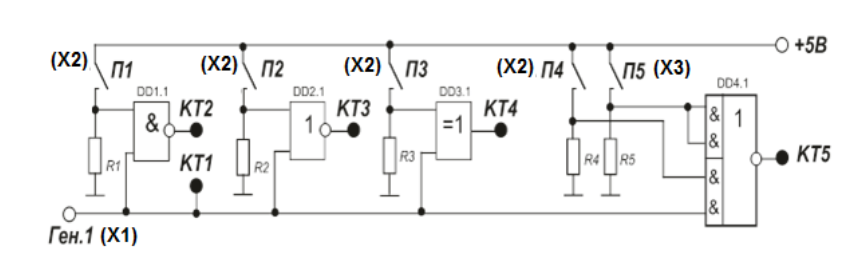
\includegraphics[width=0.8\linewidth]{1.png}}
	\caption{Схеми комбiнацiйних елементiв, якi дослiджуються в лабораторнiй роботi.}
	\label{ris1}
\end{figure}

На рис.1 представленi дослiджуванi схеми комбiнацiйних елементiв. Елемент
DD1.1 реалiзує функцiю I-НI, елемент DD2.1 - функцiю АБО-НI, елемент DD3.1
-ВИКЛЮЧАЮЧЕ-АБО, елемент DD4.1 – функцiю 2-I-АБО-НI. Перемикачi П1 -
П5 задають вхiднi сигнали логiчних елементiв. Якщо перемикач не замкнений
– на вiдповiдний вхiд логiчного елемента подається рiвень логiчного нуля че-
рез пiдключення до землi. Якщо перемикач замкнений, то до вiдповiдного входу
пiд’єднується напруга живлення +5В, що вiдповiдає подачi на цей вхiд рiвня ло-
гiчної одиницi. В контрольних точках КТ2 - КТ5 спостерiгаються вихiднi сигнали
вiдповiдних логiчних елементiв.

\clearpage
\begin{center}
\fbox{Виконання роботи}
\end{center}

\begin{figure}[h]
	\center{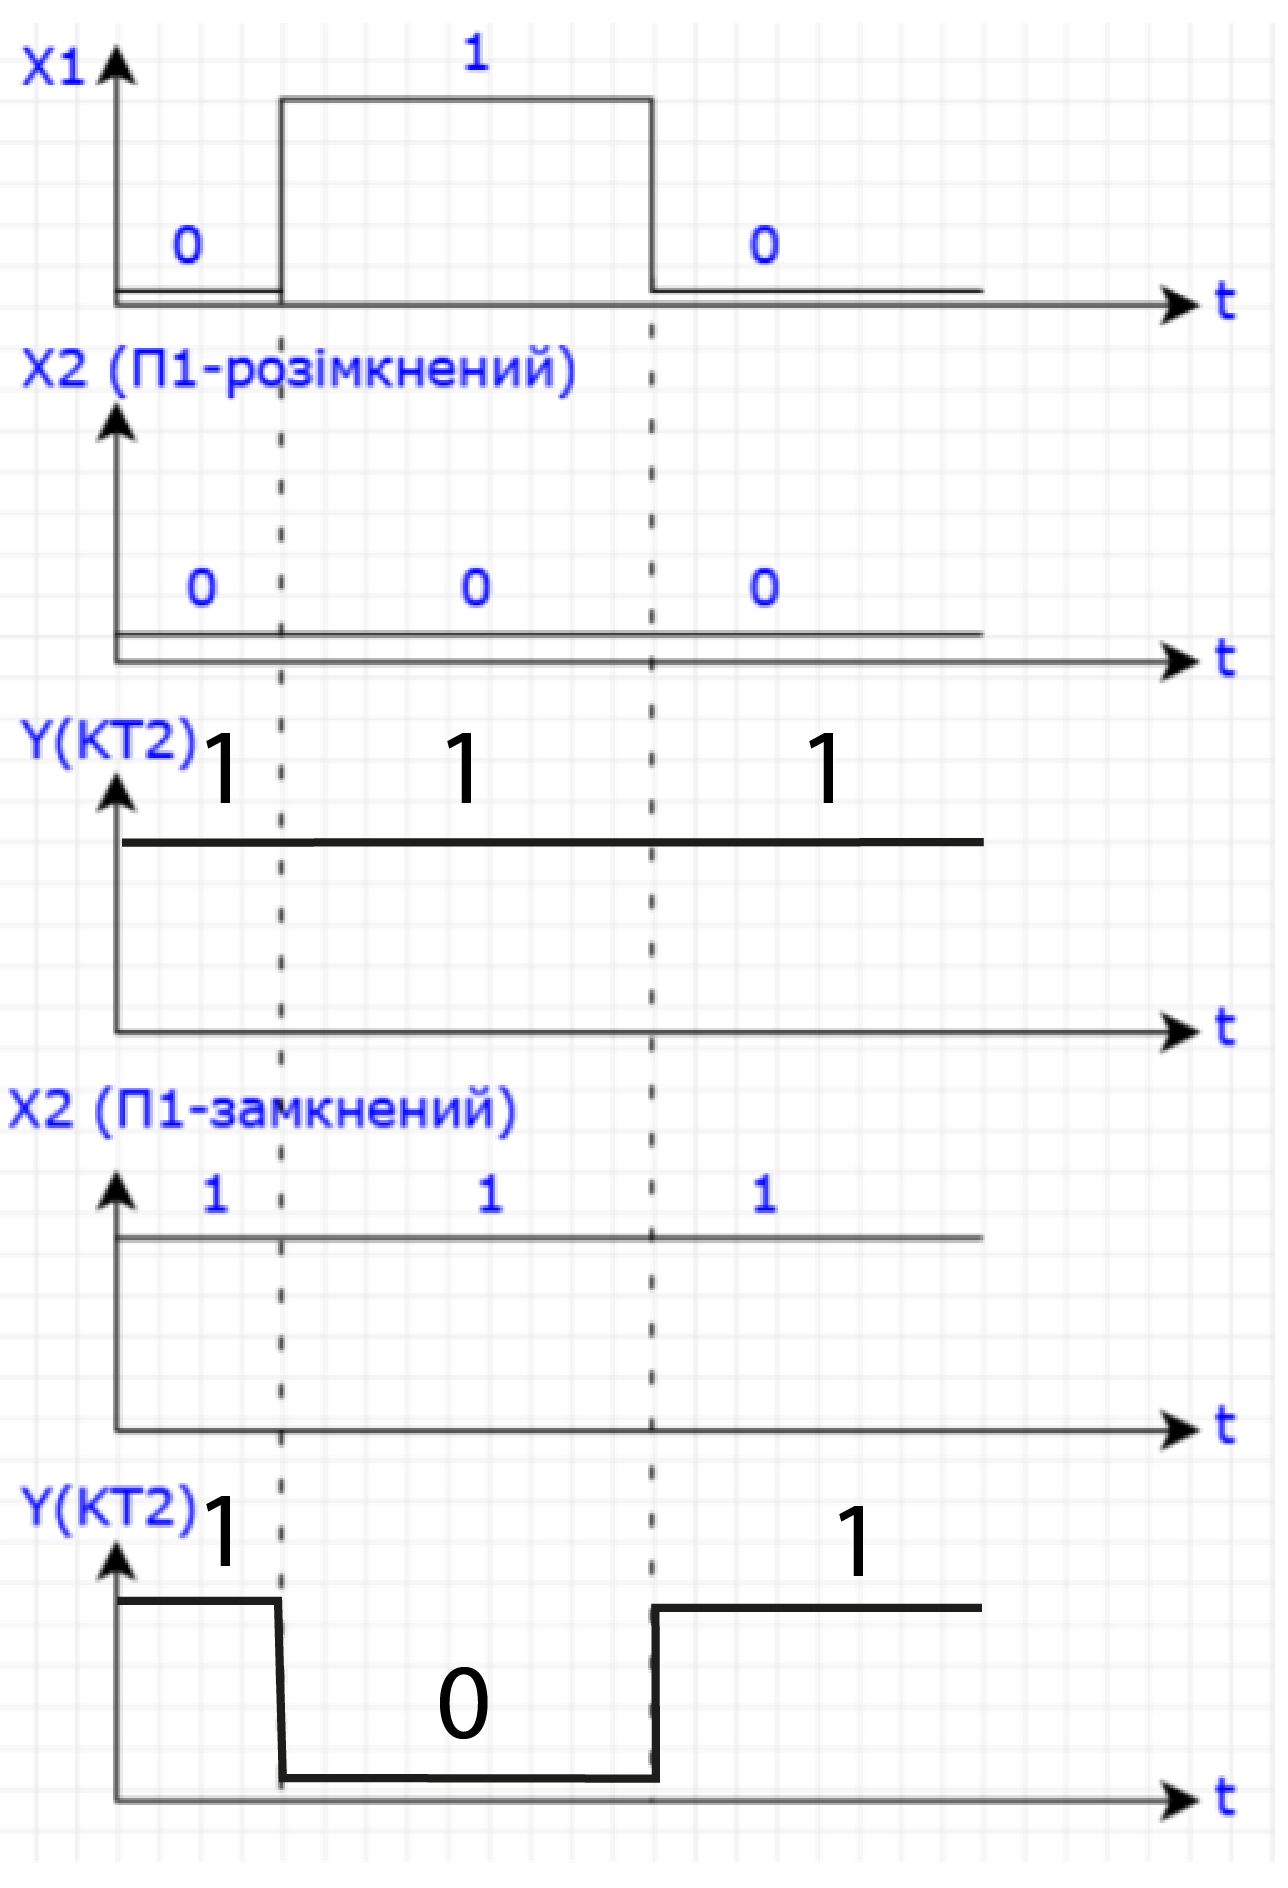
\includegraphics[width=0.5\linewidth]{2.png}}
	\caption{Часові діаграми роботи логічного елементу І-НІ}
	\label{ris2}
\end{figure}
\begin{table}[h!]
	\begin{center}
	\begin{tabular}{|c|c|c|c|c|}
	\hline
	x1 & 0 & 0 & 1 & 1 \\ \hline
	x2 & 0 & 1 & 0 & 1 \\ \hline
	y  & 1 & 1 & 1 & 0 \\ \hline
	\end{tabular}
	\end{center}
\end{table}


\clearpage
\begin{figure}[h]
	\center{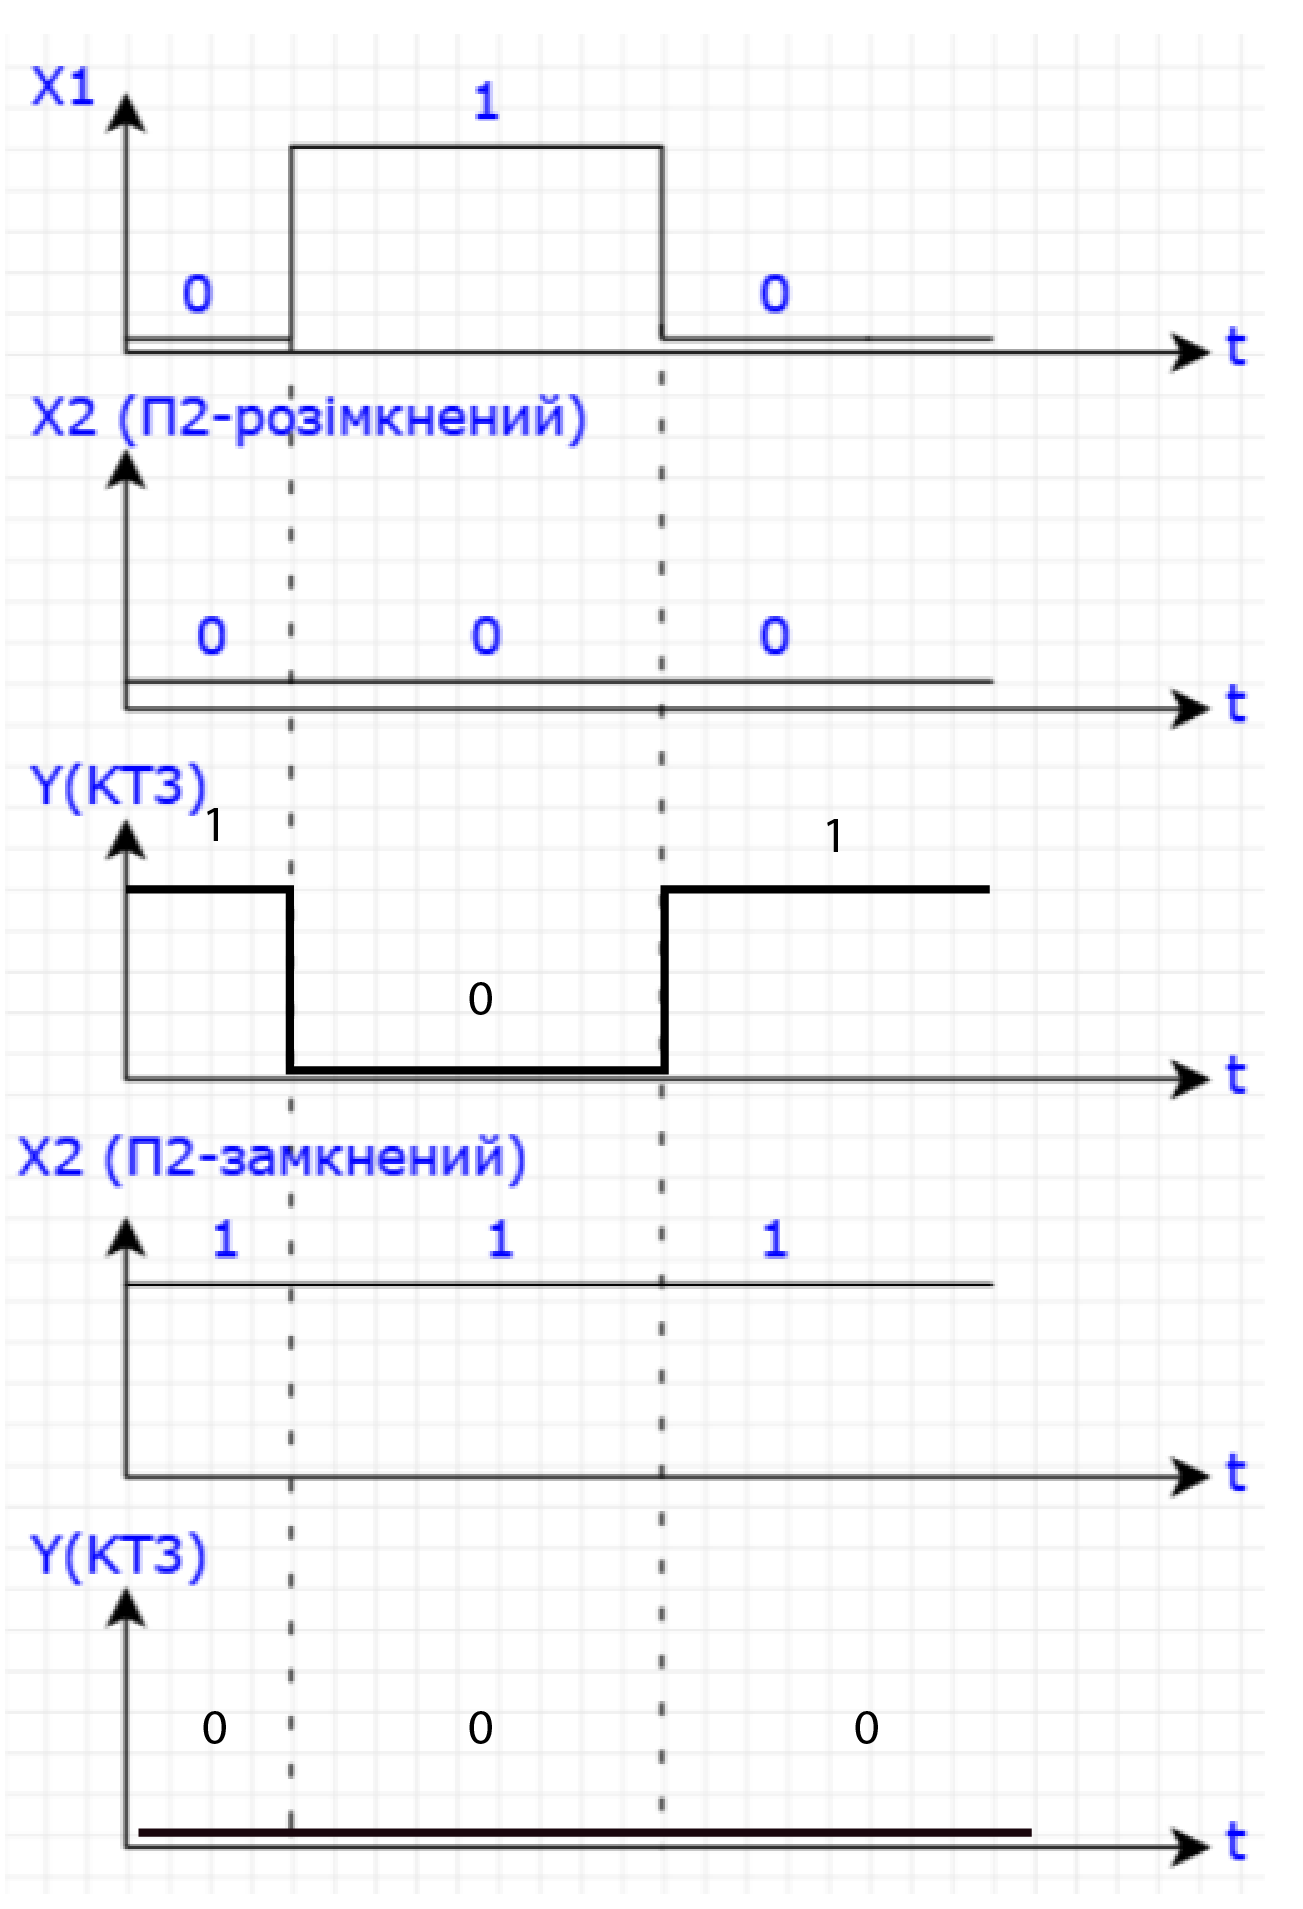
\includegraphics[width=0.6\linewidth]{3.png}}
	\caption{Часовi дiаграми роботи логiчного елементу АБО-НI}
	\label{ris2}
\end{figure}
\begin{table}[h!]
	\begin{center}
	\begin{tabular}{|c|c|c|c|c|}
	\hline
	x1 & 0 & 0 & 1 & 1 \\ \hline
	x2 & 0 & 1 & 0 & 1 \\ \hline
	y  & 1 & 0 & 0 & 0 \\ \hline
	\end{tabular}
	\end{center}
\end{table}

\clearpage
\begin{figure}[h!]
	\center{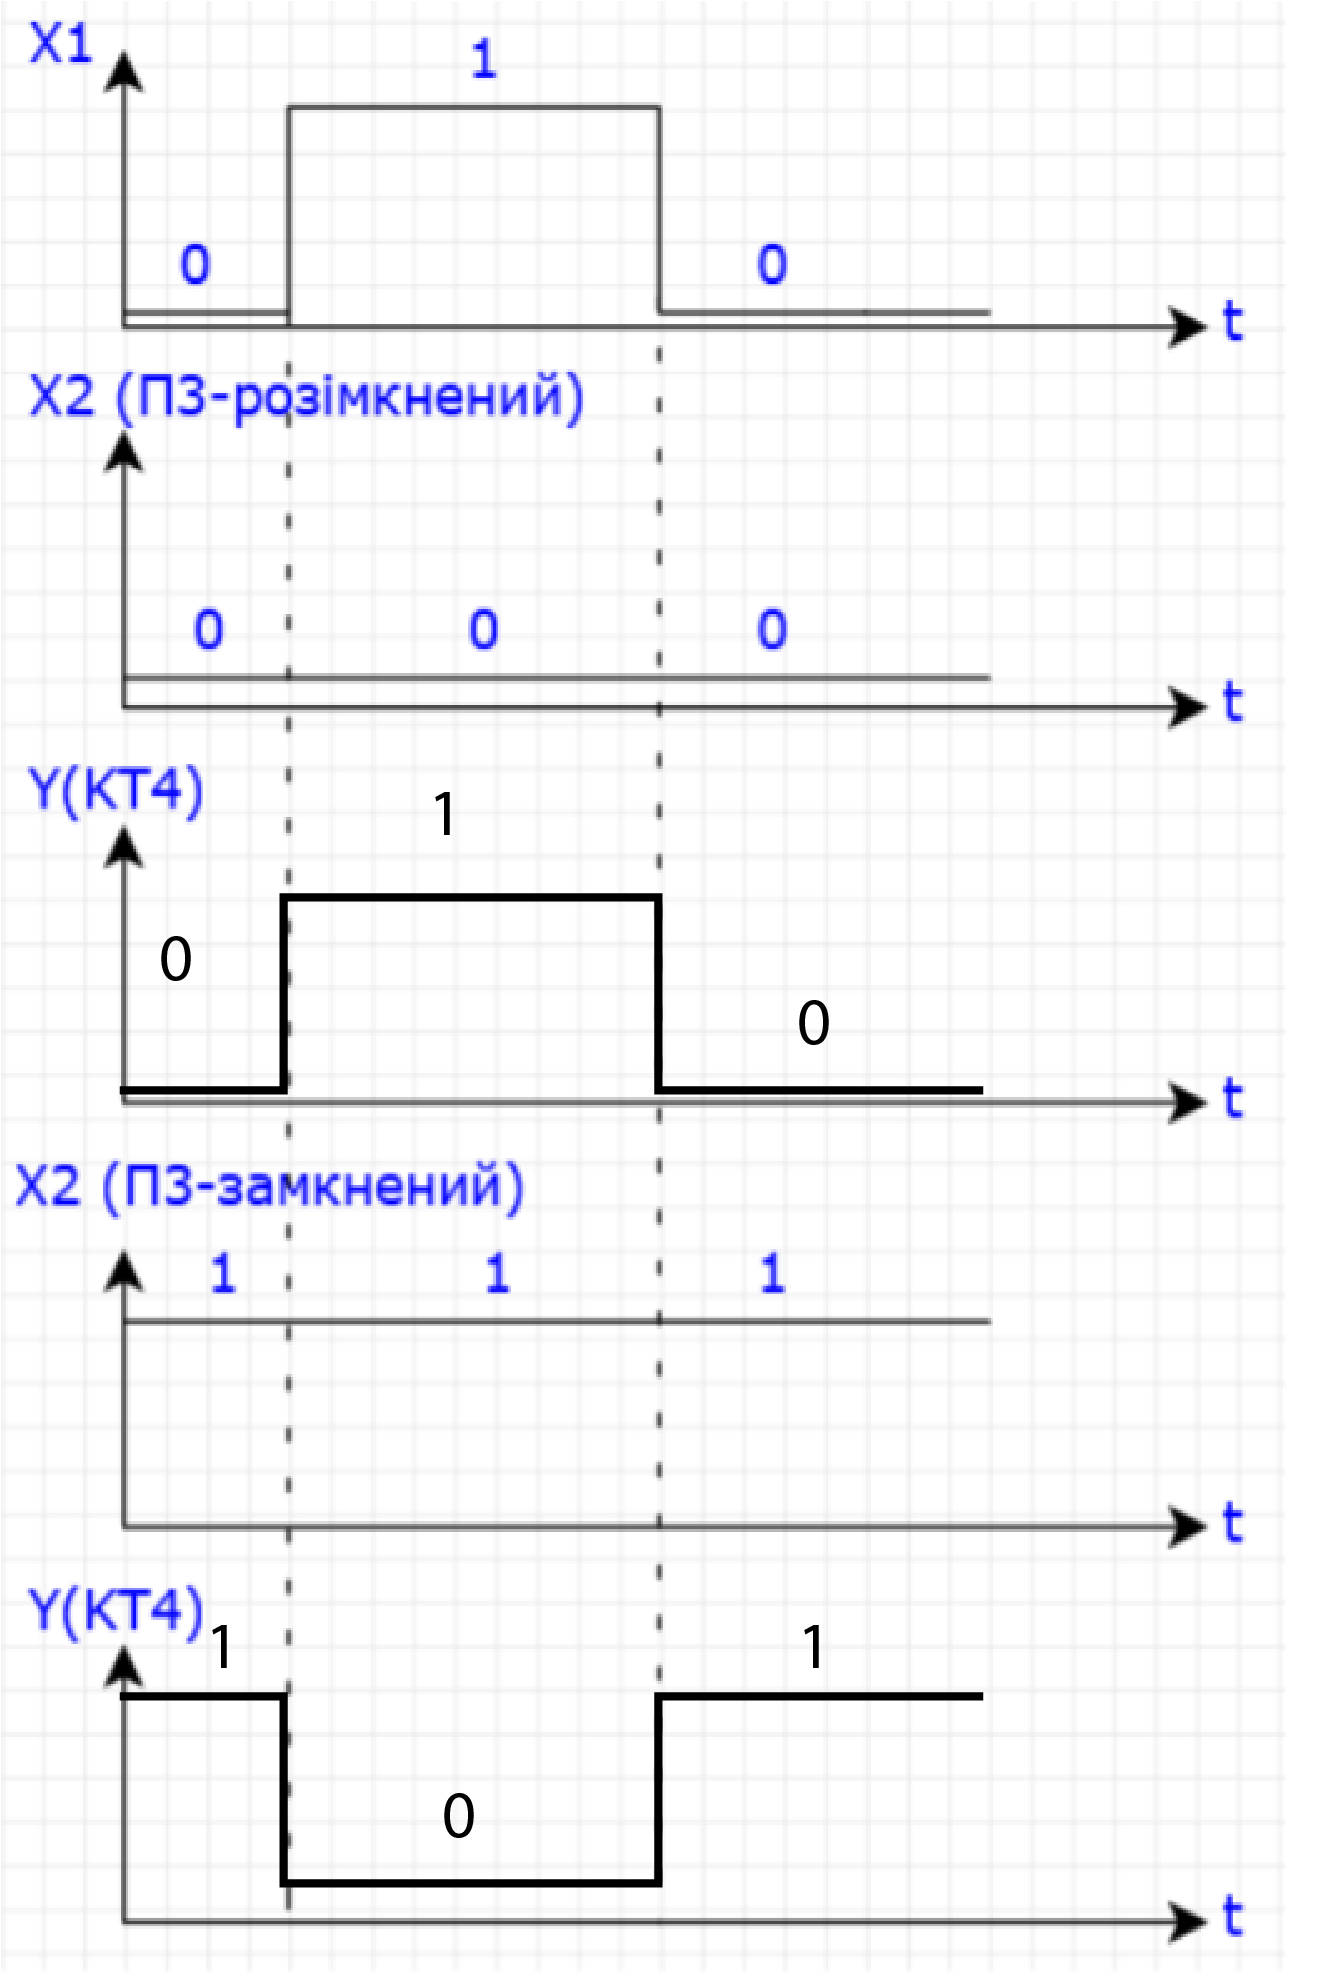
\includegraphics[width=0.6\linewidth]{4.png}}
	\caption{Часовi дiаграми роботи логiчного елементу ВИКЛЮЧНЕ АБO}
	\label{ris2}
\end{figure}
\begin{table}[h!]
	\begin{center}
	\begin{tabular}{|c|c|c|c|c|}
	\hline
	x1 & 0 & 0 & 1 & 1 \\ \hline
	x2 & 0 & 1 & 0 & 1 \\ \hline
	y  & 0 & 1 & 1 & 0 \\ \hline
	\end{tabular}
	\end{center}
\end{table}


\clearpage
\begin{figure}[h]
	\center{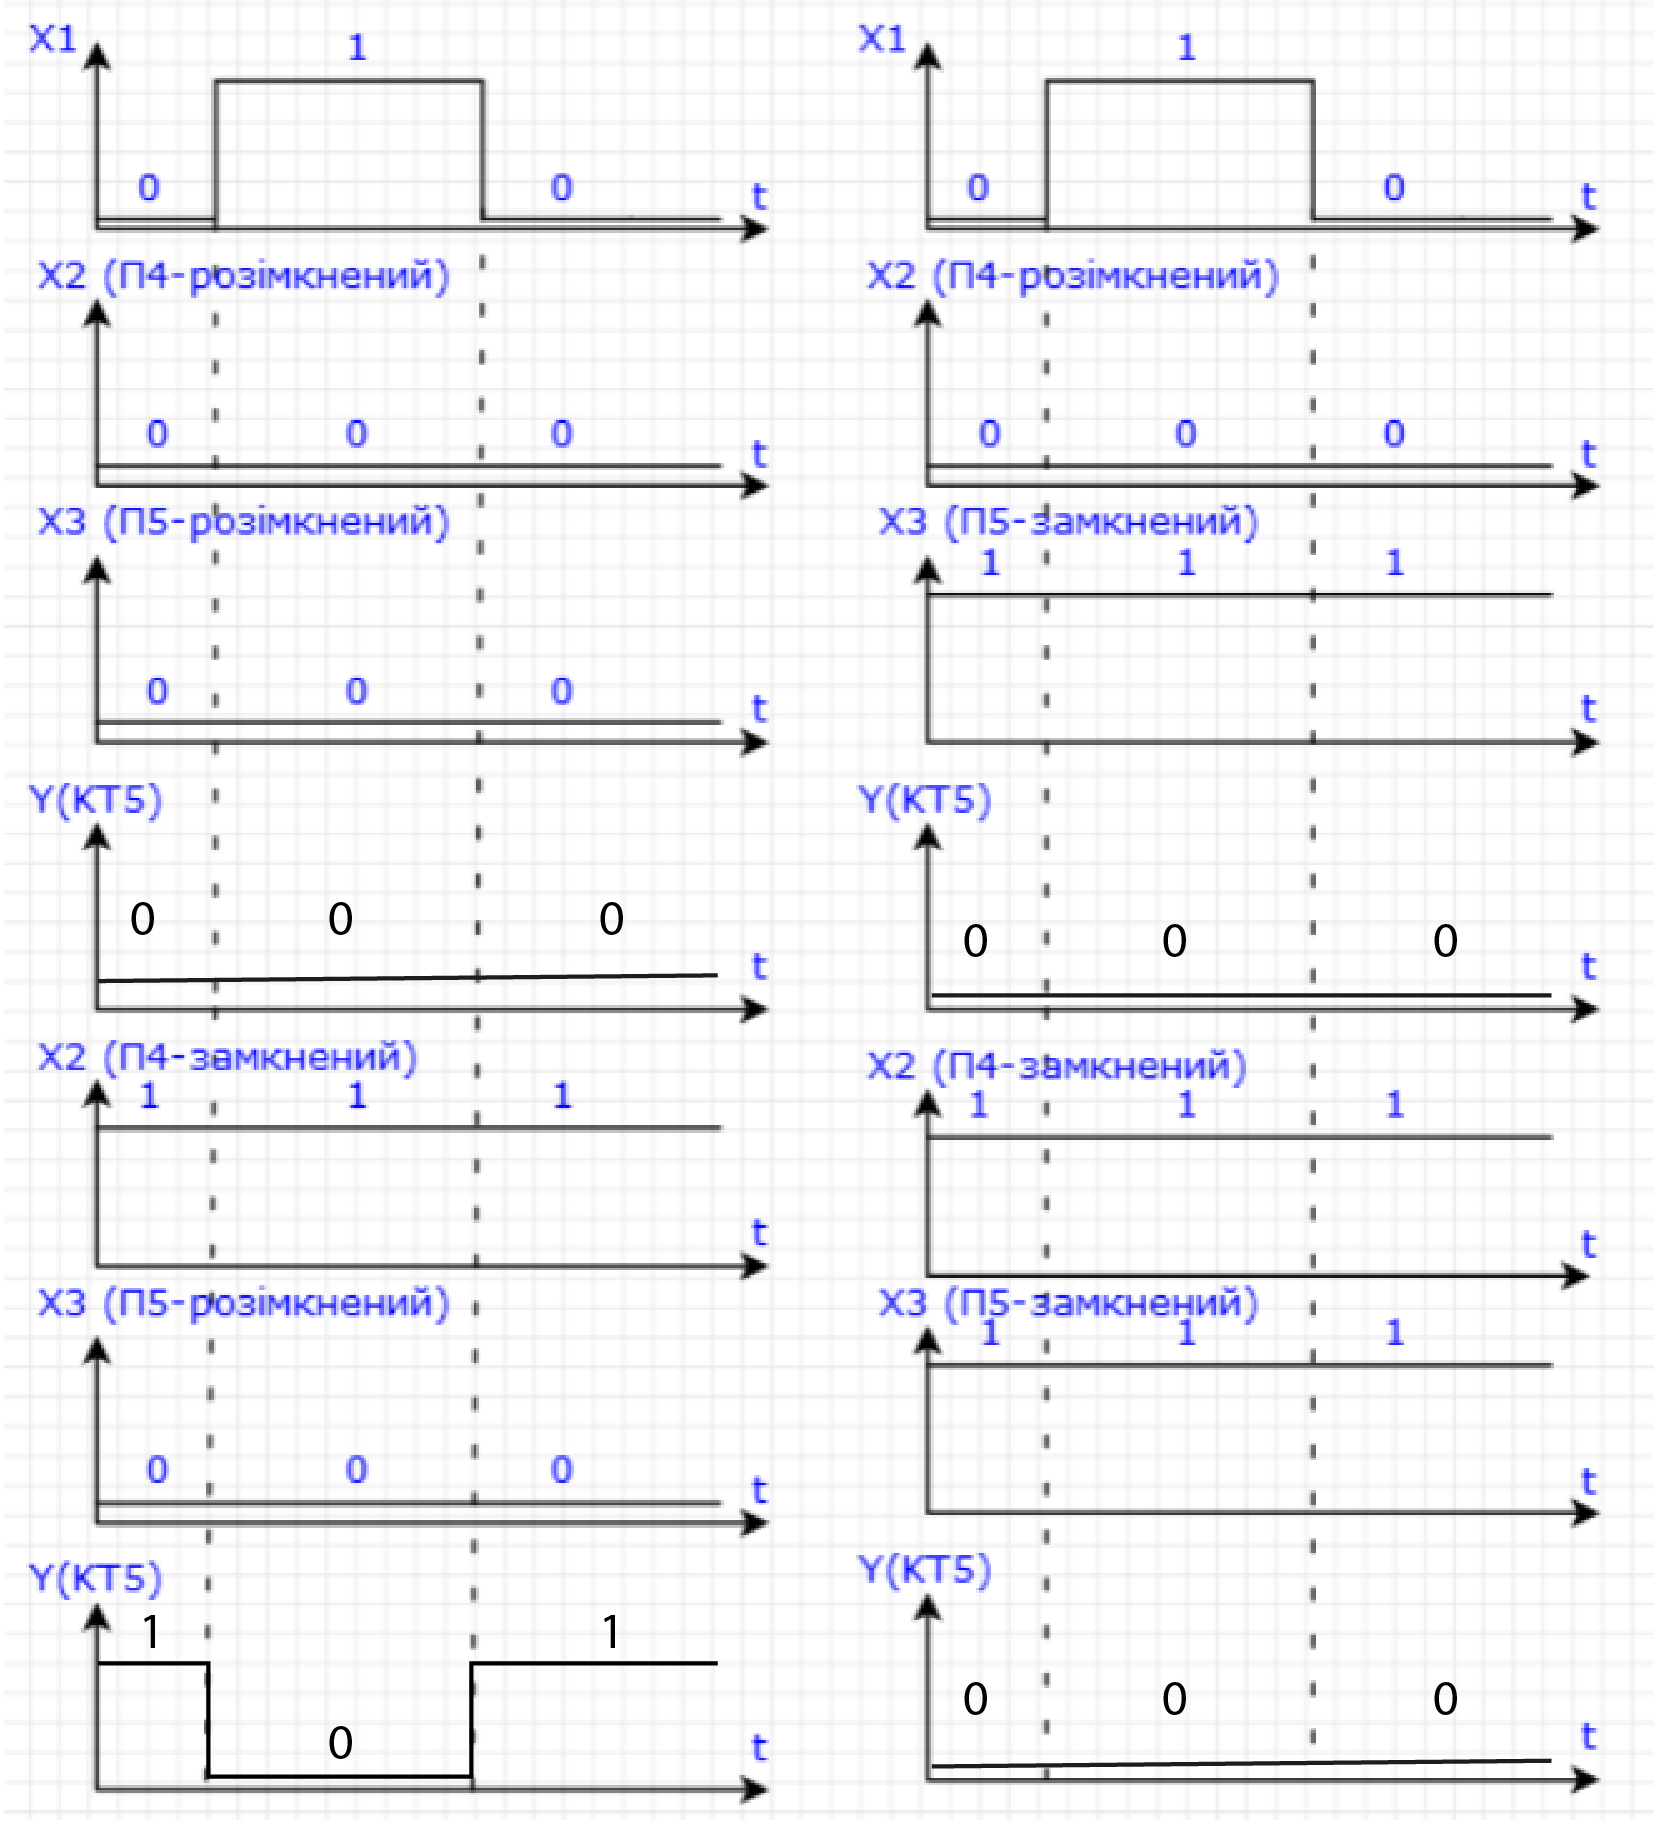
\includegraphics[width=0.8\linewidth]{5.png}}
	\caption{Часовi дiаграми роботи логiчного елементу I-АБО-НI}
	\label{ris2}
\end{figure}

\begin{table}[h!]
\begin{center}
\begin{tabular}{|c|c|c|c|c|c|c|c|c|}
\hline
x1 & 0 & 0 & 0 & 0 & 1 & 1 & 1 & 1 \\ \hline
x2 & 0 & 0 & 1 & 1 & 0 & 0 & 1 & 1 \\ \hline
x3 & 0 & 1 & 0 & 1 & 0 & 1 & 0 & 1 \\ \hline
y  & 1 & 0 & 1 & 0 & 1 & 0 & 0 & 0 \\ \hline
\end{tabular}
\end{center}
\end{table}



\clearpage
\newpage
\begin{center}
	\fbox{Визначення затримки поширення сигналiв досліджуваних ЛЕ}
	\end{center}

	\begin{equation}
	\begin{array}{|c|c|c|}
	\hline \text { ЛE } & t_{\text {з.п. }}^{01}, \text { нс } & t_{\text {з.п. }}^{10}, \text { нс } \\
	\hline \text { I-HI } & 9 & 120 \\
	\hline \text { AБO-HI } & 66 & 66 \\
	\hline \text { ВИКЛЮЧHE AБO } & 72 & 100 \\
	\hline \text { 2I-АБO-HI } & 148 & 224 \\
	\hline
	\end{array}
	\end{equation}












\clearpage 
\newpage
\begin{center}
\textbf{\fbox{Висновок}}
\end{center}
Аналізуючи дані отримані в ході лабораторної роботи можна підмітити особливості затримками поширення, наприклад у
 \textbf{ЛЕ I-НI має} --- найменшу затримку при переходi з закритого у вiдкритий стан.
\textbf{ЛЕ АБО-НI} --- має найменшу затримку при переходi з вiдкритого у закритий стан.
\textbf{ЛЕ ВИКЛЮЧНЕ АБО} не має якихось особливостей окрим того, що перемикання з закритого у вiдкритий стан вiдбувається  швидше, нiж з вiдкритого у закритий.
\textbf{ЛЕ 2-I-АБО-НI} --- має найбiльшу затримку серед усiх ЛЕ при переходi з закритого у вiдкритий стан i навпаки, пояснюється затримка тим що це просто такий елемент за своєю так би мовити каскаднiстю операцiй може накопичувіти затримку.









\end{document}